% Seção 1
\section{O que é Física?}
	A Física é a ciência que estuda os \highlight{fenômenos naturais} e as leis que regem o comportamento da \highlight{matéria} e da \highlight{energia} no universo. Seu objetivo principal é compreender e descrever como o mundo funciona.
	
	\begin{itemize}
		\item Exemplos de estudos da Física:
		\begin{itemize}
			\item Por que objetos caem (gravidade).
			\item Como a luz se comporta.
			\item O funcionamento de motores e dispositivos elétricos.
		\end{itemize}
	\end{itemize}
	
	A Física é essencial para o avanço de várias áreas, como a Química, a Biologia e a Engenharia.
	
	% Seção 2
	\section{Para que serve o estudo da Física?}
	O estudo da Física permite entender o mundo e desenvolver soluções práticas para problemas do dia a dia. Além disso, ela contribui para o desenvolvimento de tecnologias e metodologias científicas.
	
	\subsection*{Aplicações da Física}
	\begin{enumerate}
		\item \highlight{Tecnologia}: Como celulares, computadores e motores.
		\item \highlight{Saúde}: Raios X e ressonância magnética.
		\item \highlight{Engenharia}: Construção de pontes e sistemas de transporte.
		\item \highlight{Astronomia}: Exploração do espaço e estudo dos astros.
	\end{enumerate}
	
	\textbf{Além disso}, aprender Física desenvolve o pensamento lógico e crítico.
	
	% Seção 3
	\section{Grandezas físicas e unidades}
	\subsection*{Grandezas físicas}
	Grandezas físicas são características que podem ser medidas, como massa, tempo e velocidade.
	
	\subsection*{Sistema Internacional de Unidades (SI)}
	As grandezas físicas são medidas utilizando unidades padronizadas. As principais no SI são:
	\begin{itemize}
		\item \textbf{Comprimento}: metro (\(m\)).
		\item \textbf{Massa}: quilograma (\(kg\)).
		\item \textbf{Tempo}: segundo (\(s\)).
		\item \textbf{Temperatura}: kelvin (\(K\)).
	\end{itemize}
	
	% Seção 4
	\section{Notação científica}
	A \textbf{notação científica} é usada para simplificar números muito grandes ou muito pequenos, utilizando potências de 10.
	
	\subsection*{Exemplos}
	\begin{align*}
		300000000 & = 3 \times 10^8 \quad \text{(velocidade da luz)} \\
		0,00045 & = 4,5 \times 10^{-4}
	\end{align*}
	
	Essa técnica é amplamente utilizada na Física para expressar grandezas astronômicas ou microscópicas.
	
	% Seção 5
	\section{Medidas de intervalo de tempo}
	O tempo é uma grandeza física fundamental. Ele pode ser medido em diferentes escalas:
	\begin{itemize}
		\item \textbf{Segundo (\(s\))}: Unidade básica do SI.
		\item \textbf{Minuto (\(min\))}: 1 minuto = 60 segundos.
		\item \textbf{Hora (\(h\))}: 1 hora = 60 minutos.
	\end{itemize}
	
	\subsection*{Exemplos práticos}
	\begin{itemize}
		\item O tempo que a luz do Sol demora para chegar à Terra: \highlight{8 minutos}.
		\item O tempo médio de uma batida do coração humano: \highlight{1 segundo}.
	\end{itemize}
	
	% Seção 6
	\section{Medidas de comprimento}
	O comprimento mede a distância entre dois pontos. É uma das grandezas mais importantes na Física.
	
	\subsection*{Unidades de comprimento no SI}
	\begin{itemize}
		\item \textbf{Metro (\(m\))}: Unidade padrão.
		\item \textbf{Quilômetro (\(km\))}: 1 km = 1000 metros.
		\item \textbf{Centímetro (\(cm\))}: 1 cm = 0,01 metros.
		\item \textbf{Milímetro (\(mm\))}: 1 mm = 0,001 metros.
	\end{itemize}
	
	\subsection*{Unidades usadas em Astronomia}
	\begin{itemize}
		\item \textbf{Ano-luz}: Distância que a luz percorre em um ano (\(9,46 \times 10^{12} \, km\)).
		\item \textbf{Angstrom (\(Å\))}: Medida para átomos (\(1 Å = 10^{-10} \, m\)).
	\end{itemize}
	
	\subsection*{Exemplos práticos}
	\begin{itemize}
		\item Altura de uma pessoa: cerca de \(1,7 \, m\).
		\item Raio da Terra: aproximadamente \(6.371 \, km\).
		\item Distância da Terra à Lua: cerca de \(384.400 \, km\).
	\end{itemize}
	
\begin{center}
	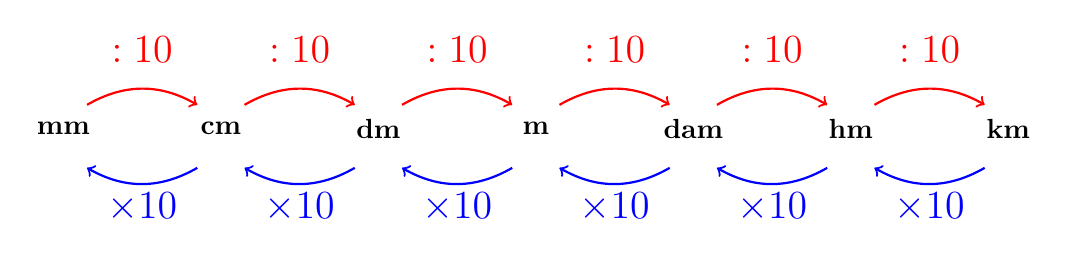
\begin{tikzpicture}
		% Definição das caixas das unidades
		\node at (0,0) {\textbf{mm}};
		\node at (2,0) {\textbf{cm}};
		\node at (4,0) {\textbf{dm}};
		\node at (6,0) {\textbf{m}};
		\node at (8,0) {\textbf{dam}};
		\node at (10,0) {\textbf{hm}};
		\node at (12,0) {\textbf{km}};
		
		% Setas curvadas para divisão por 10 (para a direita)
		\draw[->, red, thick] (0.3,0.3) to[out=30, in=150] (1.7,0.3);
		\draw[->, red, thick] (2.3,0.3) to[out=30, in=150] (3.7,0.3);
		\draw[->, red, thick] (4.3,0.3) to[out=30, in=150] (5.7,0.3);
		\draw[->, red, thick] (6.3,0.3) to[out=30, in=150] (7.7,0.3);
		\draw[->, red, thick] (8.3,0.3) to[out=30, in=150] (9.7,0.3);
		\draw[->, red, thick] (10.3,0.3) to[out=30, in=150] (11.7,0.3);
		
		% Texto sobre as setas para divisão
		\node[red] at (1,1) {\Large $:10$};
		\node[red] at (3,1) {\Large $:10$};
		\node[red] at (5,1) {\Large $:10$};
		\node[red] at (7,1) {\Large $:10$};
		\node[red] at (9,1) {\Large $:10$};
		\node[red] at (11,1) {\Large $:10$};
		
		% Setas curvadas para multiplicação por 10 (para a esquerda)
		\draw[->, blue, thick] (1.7,-0.5) to[out=210, in=-30] (0.3,-0.5);
		\draw[->, blue, thick] (3.7,-0.5) to[out=210, in=-30] (2.3,-0.5);
		\draw[->, blue, thick] (5.7,-0.5) to[out=210, in=-30] (4.3,-0.5);
		\draw[->, blue, thick] (7.7,-0.5) to[out=210, in=-30] (6.3,-0.5);
		\draw[->, blue, thick] (9.7,-0.5) to[out=210, in=-30] (8.3,-0.5);
		\draw[->, blue, thick] (11.7,-0.5) to[out=210, in=-30] (10.3,-0.5);
		
		% Texto sobre as setas para multiplicação
		\node[blue] at (1,-1) {\Large $\times 10$};
		\node[blue] at (3,-1) {\Large $\times 10$};
		\node[blue] at (5,-1) {\Large $\times 10$};
		\node[blue] at (7,-1) {\Large $\times 10$};
		\node[blue] at (9,-1) {\Large $\times 10$};
		\node[blue] at (11,-1) {\Large $\times 10$};
		
	\end{tikzpicture}
\end{center}
